%        File: report.tex
%     Created: Sun Feb 21 08:00 AM 2016 E
% Last Change: Sun Feb 21 08:00 AM 2016 E
%
\documentclass[a4paper]{report}

\usepackage{mathtools} 
\usepackage{amsmath}
\usepackage{amssymb}
\usepackage{newlfont}
\usepackage{caption}
\usepackage{subcaption}
\usepackage{titlesec}
\usepackage{graphicx}
\usepackage{empheq}

\newcommand{\eref}[1]{Eq.~(\ref{#1})}
\newcommand{\erefs}[2]{Eq.s~(\ref{#1}-\ref{#2})}

\title{Written Preliminary Exam \#1 \break
       Prepared by Dr. Hassan}

\author{ Kyle B. Thompson }

\begin{document}
\maketitle

\begin{enumerate}
  \item Constant density flow and incompressible flow are two different things.
    Constant density implies that a fluid(s) density is constant, but capable of
    changing (through compression or expansion), whereas incompressible implies
    the fluid(s) density is incapable of changing but that the density in the
    flow is not constant.  A good example from the MAE 560 course to distinguish
    the two is stagnant air in a room, versus an oil/water mixture.  Stagnant
    air in a room is at constant density, but is certainly capable of both
    compression or expansion; therefore, it is a constant density flow, but not
    incompressible.  An oil/water mixture is not constant density.  As
    illustrated in figure \ref{fig:incompressible},the
    water and oil are different fluids with different densities, but the fluids
    are incompressible because both the water and oil are not capable of
    compression or expansion (at least in a practical sense); therefore, it not
    a constant density flow, but is incompressible.

    \begin{figure}[h]
      \centering
      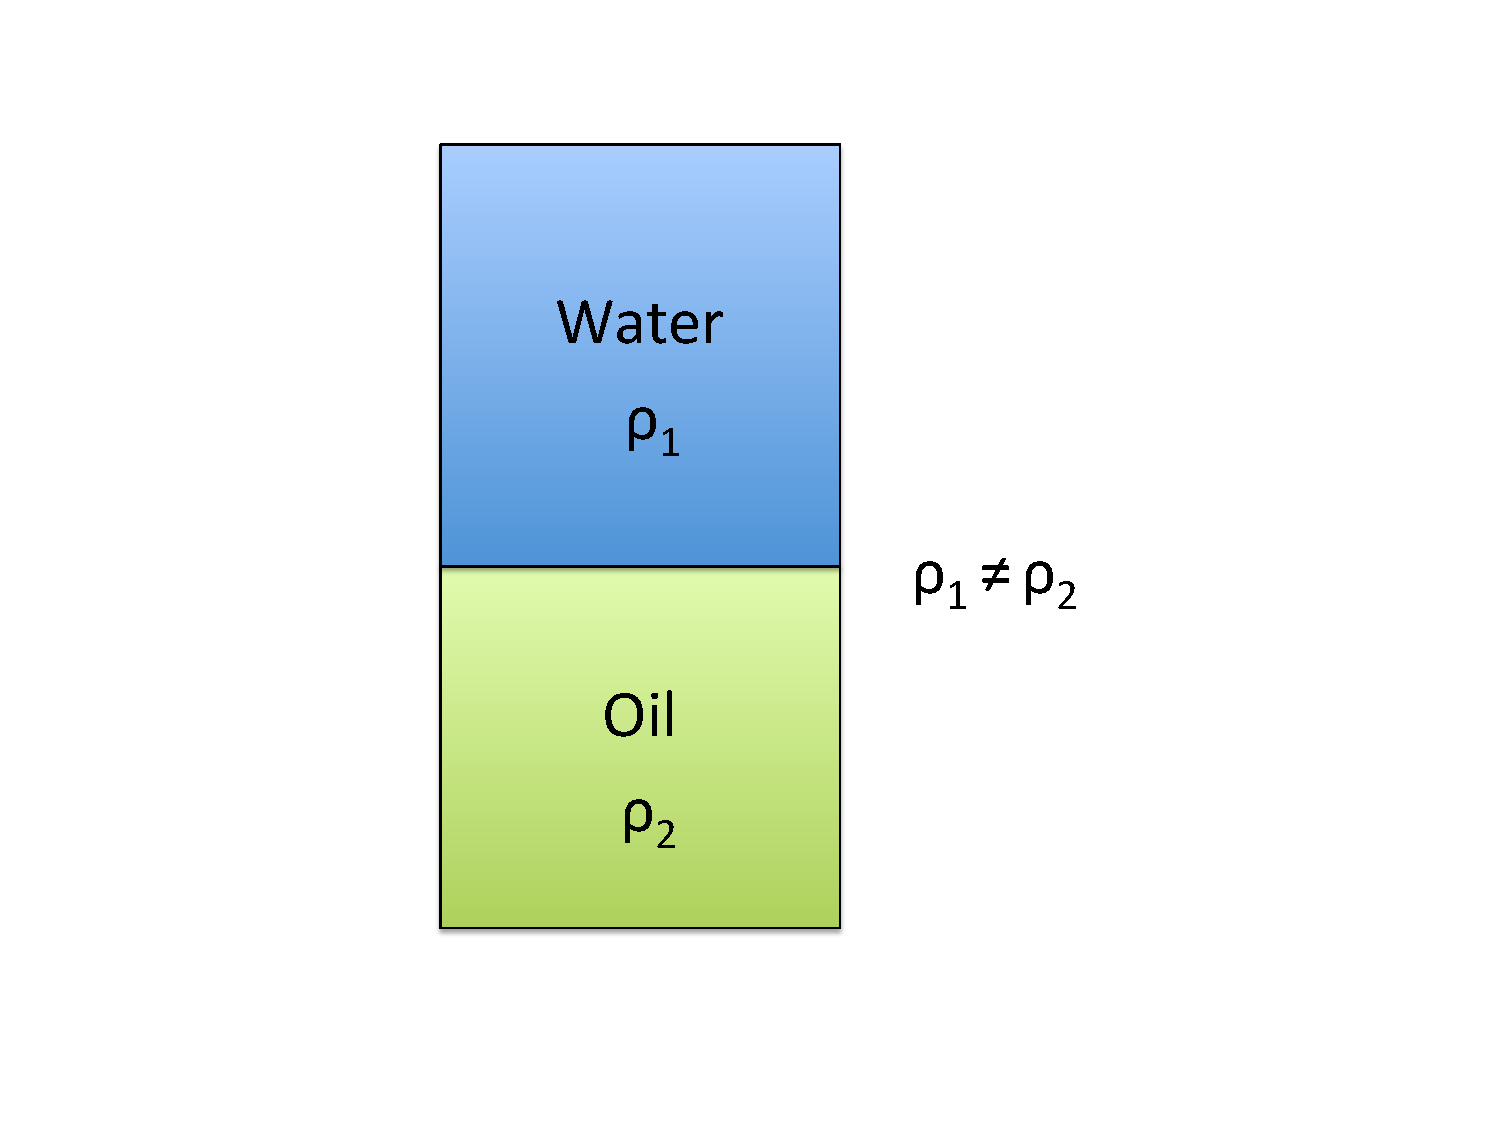
\includegraphics[width=0.8\textwidth,trim={0 2cm 0 2cm},clip]{oil_water_fig}
      \caption{Incompressible Fluid Flow Example}
      \label{fig:incompressible}
    \end{figure}

  \item There are many ways to derive an expression for change in entropy.  From
    a classical thermodynamics perspective, this comes from the definition of
    Gibbs free energy, $G$
    \begin{equation}
      G = H - TS
      \label{gfe-def}
    \end{equation}
    Where $H$ is enthalpy, $T$ is temperature, and $S$ is entopy.  It is
    straightforward to see that the first and second laws of thermodynamics can
    be used to determine the change of entropy
    \begin{align}
      dQ &= dH - VdP \label{1st-law}\\
      dS &= \frac{dQ}{T} + dS_{i}= \frac{dH - Vdp}{T} + dS_{i}
      \label{2nd-law}
    \end{align}
    Where $dS_i$ is entropy generated from ireversible processes. Using the
    definition of the enthalpy \begin{equation}
      H = E + pV
      \label{enthalpy-def}
    \end{equation}
    \eref{2nd-law} can be expanded as
    \begin{equation}
      \begin{aligned}
	dS &= \frac{dE + pdV + Vdp - Vdp}{T} + dS_i\\
	   &= \frac{dE + pdV}{T} + dS_i
      \end{aligned}
      \label{s-one-gas}
    \end{equation}
    While this is useful, this derivation is deficient as it does not account
    for multiple species in chemical non-equilibrium.  Revisiting Gibbs free
    energy for multiple species, if a system is considered for each isolated
    species then
    \begin{equation}
      G_s = G_s(p,T,N_s)
      \label{G-species-def}
    \end{equation}
    and differentiating yields
    \begin{equation}
      dG_s = \left( \frac{\partial G_s}{\partial T} \right)_{(p,N_s)} dT
      + \left( \frac{\partial G_s}{\partial p} \right)_{(T,N_s)} dp
      + \left( \frac{\partial G_s}{\partial N_s} \right)_{(p,T)} dN_s
      \label{G-species-diff}
    \end{equation}
    Where $G_s$ is the Gibbs free energy of the isolated species $s$. Because 
    $G = \sum\limits_{\substack{s=1}}^{N_{ns}}{G_s}$, \eref{G-species-diff} can
    be written as
    \begin{equation}
      dG = \left( \frac{\partial G}{\partial T} \right)_{(p,N_s)} dT
      + \left( \frac{\partial G}{\partial p} \right)_{(T,N_s)} dp
      + \sum\limits_{s=1}^{N_{ns}}{\left( \left( \frac{\partial G}{\partial N_s}
      \right)_{(p,T)} dN_s\right)}
      \label{G-diff}
    \end{equation}
    Introducing the concept of chemical potential
    \begin{equation}
      \mu_s = \left( \frac{\partial G}{\partial N_s} \right)_{p,T}
      \label{mu-def}
    \end{equation}
    and writing \eref{gfe-def} in differential form and substituting
    \eref{s-one-gas} yields
    \begin{equation}
      \begin{aligned}
        dG &= dH - SdT - TdS \\
	&= dH - SdT - T\left( \frac{dH - Vdp}{T} + dS_i \right) \\
	&= Vdp - SdT - TdS_i
      \end{aligned}
      \label{G-def-diff}
    \end{equation}
    It is clear that in comparing \eref{G-def-diff} and \eref{G-diff} that
    \begin{equation}
      \left( \frac{\partial G}{\partial T} \right)_{(p,N_s)} = V, \quad
      \left( \frac{\partial G}{\partial p} \right)_{(T,N_s)} = S, \quad
      \label{G-derivs}
    \end{equation}
    and most importantly
    \begin{equation}
      dS_i = -\frac{1}{T}\sum\limits_{s=1}^{N_{ns}}{\mu_s dN_s}
      \label{si-def}
    \end{equation}
    Thus, it is now clear that the change of entropy is defined in two
    components: the entropy generated by reversible processes, $S_r$, and the
    entropy generated by irreversible processes, $S_i$.  If \eref{G-def-diff} is
    expanded with $dS_i = 0$ and the definition of enthalpy in
    \eref{enthalpy-def} is used, the entropy from reversible processes is given
    by
    \begin{equation}
      dS_r = \frac{dE}{T} + \frac{pdV}{T}
      \label{sr-def}
    \end{equation}
    combining \erefs{si-def}{sr-def} the change of entropy expression is
    obtained
    \begin{equation}
      \boxed{dS = \frac{dE}{T} + \frac{pdV}{T} 
      -\frac{1}{T}\sum\limits_{s=1}^{N_{ns}}{\mu_s dN_s}}
      \label{ds-final}
    \end{equation}
    
    If two gases with the same pressure and temperature are mixed, then
    \eref{ds-final} shows that entropy must be generated, regardless of whether
    chemical reactions occur.  Since entropy of a system of gases is additive,
    \begin{equation}
      dS_{mix} = dS_1 + dS_2
      \label{s-additive}
    \end{equation}
    where $dS_{mix}$ is the change of entropy in the mixture, and $dS_{(1,2)}$
    are the changes in entropy of species being mixed.  There is no change in
    temperature or pressure, so $dE = 0$ for both species; however, the volume
    has changed, so for intert gases mixing there will be production of entropy
    \begin{equation}
      dS_{mix} = \frac{p}{T}\left( dV_1 + dV_2 \right)
      \label{smix-change}
    \end{equation}
    Where $dV_1$ and $dV_2$ are the changes in volume for species 1 and 2,
    respectively.  The production of entropy is to be expected, intuitively,
    since the diffusion of one gas into the other happens spontaneously.  Each
    gas will expand into the new volume available after mixing naturally, and it
    takes effort to separate them; hence $dS_mix > 0$.  Likewise, if chemical
    reactions occur, entropy will also be generated as dictated by
    \eref{si-def}.

\end{enumerate}

\end{document}


